\subsection*{Partie I.}
\begin{enumerate}
 \item
 \begin{enumerate}
   \item Le nombre complexe $j$ est défini comme la solution de partie imaginaire positive de l'équation $1 + z + z^2=0$. On sait aussi que
\[
  j = -\frac{1}{2} + i \frac{\sqrt{3}}{2} = e^{\frac{2i \pi}{3}},\hspace{0.5cm} j^3 = 1, \hspace{0.5cm} j^2 = \overline{j} = \frac{1}{j}, \hspace{0.5cm} |j| = 1.
\]
Comme $j^2$ est le conjugué de $j$:
\[
\frac{j^2 - j}{\overline{j^2 - j}} = \frac{\overline{j} - j}{j - \overline{j}} = -1.
\]
   \item  Avec les propriétés précédentes $|1-j| = |\overline{1-j}| = |1 - j^2|$ et $|1-j| = |j||1-j| = |j-j^2|$. On peut montrer que c'est $\sqrt{3}$.\newline
En multipliant par $u$, les modules sont multipliés par $|u|$ et les égalités sont conservées:
\begin{displaymath}
 |u-ju| = |ju-j^2u|=|j^2u -u|=\sqrt{3}|u|
\end{displaymath}
ce qui entraine que le triangle formé par les points d'affixes $u$, $ju$, $j^2u$ est équilatéral.

 \end{enumerate}

 \item
 \begin{enumerate}
   \item L'affixe du milieu de $M M'$ est $\frac{m + m'}{2}$. Comme $M$ et $M'$ sont symétriques, ce point est sur la droite $(A,B)$ donc il existe $\lambda$ réel tel que
\[
  \text{milieu de } MM' = A + \lambda \overrightarrow{AB} \Rightarrow
  \frac{m + m'}{2} = a + \lambda(b-a) \Rightarrow m + m' = 2a + 2 \lambda(b-a).
\]

   \item De manière analogue, $\overrightarrow{M M'}$ est orthogonal à $\overrightarrow{AB}$ car les points sont symétriques par rapport à $(AB)$. Cela se traduit par 
\[
  \frac{m' - m}{b-a} \in i \R \Rightarrow \exists \mu \in \R \text{ tq } m' - m = \mu i(b-a).
\]

   \item En ajoutant et en soustrayant les deux relations précédentes, on obtient
\[
\left\lbrace  
\begin{aligned}
  m' &= a + \lambda(b-a) + i \mu \frac{b-a}{2} \\
  m  &= a + \lambda(b-a) - i \mu \frac{b-a}{2}
\end{aligned} \right.
\Rightarrow
\left\lbrace 
\begin{aligned}
  \frac{m'-a}{b-a} &= \lambda + i  \frac{\mu}{2} \\
  \frac{m-a}{b-a}  &= \lambda - i \frac{\mu}{2}
\end{aligned} \right.
\Rightarrow \frac{m'-a}{b-a} = \overline{\left(\frac{m-a}{b-a}\right)}
\]
car $\lambda$ et $\mu$ sont réels.
 \end{enumerate}
 \item
 \begin{enumerate}
   \item Les relations $s(a)=a$ et $s(b)=b$ se traduisent par un système de deux équations aux inconnues $w_1$ et $w_2$
\[
  \left\lbrace
  \begin{aligned}
    \overline{a}\, w_1 + w_2 &= a \\ \overline{b}\,w_1 + w_2 &= b
  \end{aligned}
\right. .
\]
Son discriminant est
\[
  D = 
  \begin{vmatrix}
    \overline{a} & 1 \\ \overline{b} & 1
  \end{vmatrix}
= \overline{a} - \overline{b} \neq 0.
\]
Il admet un unique couple solution donné par les formules de Cramer
\[
  ( 
  \frac{
    \begin{vmatrix}
      a & 1 \\ b & 1
    \end{vmatrix}
  }{D} , 
  \frac{
    \begin{vmatrix}
      \overline{a} & a \\ \overline{b} & b
    \end{vmatrix}
  }{D} )
  = (\frac{a - b}{\overline{a - b}}, \frac{\overline{a}b - \overline{b}a}{\overline{a - b}}).
\]

   \item Pour exprimer $\frac{z' - a}{b -a}$, utilisons $m'=s(m)$, $a=s(a)$ et $b=s(b)$. \newline
   Comme $s(z) = w_1z + w_2$, les $w_2$ disparaissent dans les différence et il vient
\[
  \frac{z' - a}{b -a} = \frac{w_1 \bar{z} - w_1\bar{a}}{w_1 \bar{b} - w_1\bar{a}} = \overline{\left( \frac{z-a}{b-a}\right)}.
\]
Il s'agit de la même relation que celle obtenue en question 1 en échangeant $m$ et $z$. Les points $Z$ et $Z'$ sont donc symétriques par rapport à $(AB)$.
 \end{enumerate}
\end{enumerate}

\subsection*{Partie II.}
\begin{enumerate}
 \item Calculons les points demandés à partir de la relation de la question I.1.c. Présentons les résultats dans un tableau 
\begin{center}
\renewcommand{\arraystretch}{1.8}
\begin{tabular}{|c|c|c|c|} \hline
$(OA)$   & $(OB)$   & $(OC)$   & $(BC)$\\ \hline
$\frac{m_1-0}{1-0} = \overline{\left(\frac{m-0}{1-0}\right)}$ & 
$\frac{m_2-0}{j-0} = \overline{\left(\frac{m-0}{j-0}\right)}$ & 
$\frac{m_3-0}{j^2-0} = \overline{\left(\frac{m-0}{j^2-0}\right)}$ & 
$\frac{m_4-j}{j^2-j} = \overline{\left(\frac{m-j}{j^2-j}\right)}$\\ \hline
$m_1 = \overline{m}$ & $m_2 = j^2\, \overline{m}$ & $m_3 = j\,\overline{m}$ & $m_4 = -\overline{m} -1 $ \\ \hline
\end{tabular}
\end{center}
Certains calculs intermédiaires ont été effectués. par exemple
\[
  \frac{j}{\overline{j}} = \frac{j^4}{j^2} = j^2,\hspace{0.3cm}
  \frac{j^2}{\overline{j^2}} = \frac{j^2}{j} = j,\hspace{0.3cm}
  \frac{j^2 - j}{\overline{j^2 - j}} = \frac{\overline{j} - j}{j - \overline{j}} = -1.
\]
Les expressions de $m_1$, $m_2$, $m_3$ et la question I.1.b montrent que les points $M_1$, $M_2$, $M_3$ forment un triangle équilatéral.

\item On va montrer que $M_2$, $M_3$, $M_4$ sont alignés si et seulement si $M$ est sur le cercle de rayon $1$ et de centre le point d'affixe $-1$.\newline
Pour étudier la condition d'alignement de $M_2$, $M_3$, $M_4$ formons $\frac{m_2-m_4}{m_3-m_4}$ et utilisons la relation $1+j+j^2=0$ :
\begin{multline*}
 \frac{m_2-m_4}{m_3-m_4} = \frac{j^2\overline{m}+\overline{m}+1}{j\overline{m}+\overline{m}+1} 
= \frac{-j\overline{m}+1}{-j^2\overline{m}+1} \\ 
= \frac{1-jm -j\overline{m}+j^2|m|^2}{|-j^2\overline{m}+1|^2}
= \frac{1-2j\Re(m)+j^2|m|^2 }{|-j^2\overline{m}+1|^2}
\end{multline*}
Avec $x=\Re(m)$ et $y=\Im(m)$, l'expression précédente est réelle si et seulement si sa partie imaginaire est nulle c'est à dire:
\begin{displaymath}
 0=-\sqrt{3}x-\frac{\sqrt{3}}{2}(x^2+y^2) \Leftrightarrow (x+1)^2 + y^2 = 1
\end{displaymath}
ce qui démontre le résultat annoncé.\newline
Pour vérifier que $A$ est sur la droite, on considère la condition d'alignement de $A$ (d'affixe $1$) avec $M_2$ et $M_3$:
\[
 \frac{m_2 - 1}{m_3 - 1} = \frac{j^2 \overline{m} -1}{j \overline{m} -1} = \frac{m_3 - m_4}{m_2 - m_4} \in \R. 
\]
Ceci montre que $A$ est sur la même droite comme la figure de l'énoncé semble l'indiquer.

\item \begin{enumerate}
 \item Ici $M_2$, $M_3$, $M_4$ ne sont pas alignés et $\Omega$ est le centre du cercle circonscrit. On va prouver que $\Omega$ est  sur la droite $(OM_1)$ en montrant que $(OM_1)$ est la médiatrice de $M_2$ et $M_3$.\newline
Il suffit de montrer que $O$ et $M_1$ sont sur cette médiatrice. Comme $m_2=j^2\overline{m}$ et $m_3=j\overline{m}$, ils ont le même module donc le point $O$ est sur la médiatrice de $M_2$ et $M_3$.\newline
De même :
\begin{displaymath}
 |m_1 - m_2|=|1-j^2||m| = |1-\overline{j}||m| = |1-j||m| = |m_1-m_3| 
\end{displaymath}
donc $M_1$ est sur la médiatrice de de $M_2$ et $M_3$.

\item On note ici $m=\rho e^{i\theta}$ $\omega$ l'affixe de $\Omega$. Comme $\Omega\in (OM_1)$, il existe un réel $\lambda$ tel que $\omega=\lambda e^{-i\theta}$. \'Ecrivons que $|\omega-m_3|=|\omega-m_4|$, cela entraine :
\begin{multline*}
 |\lambda e^{-i\theta} -j\rho e^{-i\theta}| = |\lambda e^{-i\theta}+1 +\rho e^{-i\theta}| \Leftrightarrow
|\lambda -j\rho| = |\lambda+\rho +e^{i\theta}| \\
\Leftrightarrow (\lambda + \frac{\rho}{2})^2 + \frac{3}{4}\rho^2 = (\lambda + \rho + \cos \theta)^2 + \sin^2\theta \\
\Leftrightarrow  \lambda(\rho + 2\cos\theta)+1+2\rho\cos \theta = 0
\end{multline*}
d'où l'expression de $\lambda$ et celle de $\omega$ demandée par l'énoncé.

\item Pour calculer $R$, on utilise le point $M_3$.
\begin{multline*}
 R = |m_3-\omega| = \left\vert j\rho e^{-i\theta} + \frac{1+2\rho\cos \theta}{\rho +2\cos \theta}e^{-i\theta}\right\vert
= \left\vert j\rho  + \frac{1+2\rho\cos \theta}{\rho +2\cos \theta}\right\vert\\
\Rightarrow R^2 
= \rho^2 + \left(\frac{1+2\rho\cos \theta}{\rho +2\cos \theta}\right)^2 + 2\rho\,\frac{1+2\rho\cos \theta}{\rho +2\cos \theta}\Re(j)\\
= \rho^2 + \left(\frac{1+2\rho\cos \theta}{\rho +2\cos \theta}\right)\left( \frac{1+2\rho\cos \theta}{\rho +2\cos \theta} - \rho\right)
= \rho^2 + \frac{(1 + 2\rho\cos \theta)(1-\rho^2)}{(\rho + 2\cos \theta)^2}.
\end{multline*}
\end{enumerate}

\item On va montrer que $\Gamma$ est l'union du cercle unité et de la droite $(BC)$.\newline
Le cercle circonscrit aux points $M_1$, $M_2$, $M_3$ d'affixes $m_1 = \overline{m}$, $m_2 = j^2\overline{m}$ , $m_3 = j\overline{m}$ est de centre $O$ et de rayon $|m|=\rho$. D'après la question 3.c., les rayons des deux cercles circonscrits sont égaux si set seulement si :
\begin{displaymath}
 R^2 = \rho^2 \Leftrightarrow \frac{(1+2\rho\cos\theta)(1-\rho^2)}{(\rho+2\cos \theta)^2} = 0
\end{displaymath}
c'est à dire si et seulement si on est dans une des deux situations suivantes:
\[
\begin{aligned}
  &1+2\rho\cos\theta = 1+2x=0 &\Leftrightarrow& M \in (BC)\\
  &\rho =1 &\Leftrightarrow& M \text{ sur le cercle unité}.
\end{aligned}
\]
On remarque de plus que dans le premier cas, $M = M_4$ car $M \in (BC)$ et $\Omega= O$ d'après la question 3.b. Les deux cercles circonscrits ont le même centre et le même rayon, ils sont confondus.\newline
La figure 4 complétée en figure \ref{fig:Ccomp2_1} présente le cas où $M$ est à sur $(BC)$. Dans ce cas les deux cercles sont confondus (de centre $O$).
\begin{figure}
 \centering
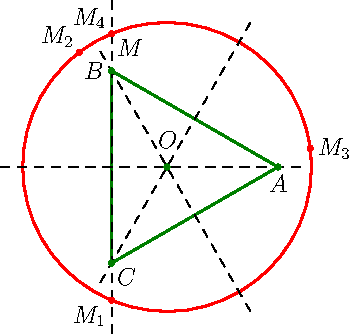
\includegraphics[width=5cm]{Ccomp2_1.pdf}
\caption{$M\in (BC)$} \label{fig:Ccomp2_1}
\end{figure} \newline
La figure 5 complétée en figure \ref{fig:Ccomp2_2} présente le cas où $M$ est sur le cercle unité. Les deux cercles sont alors de même rayon mais distincts.
\begin{figure}
 \centering
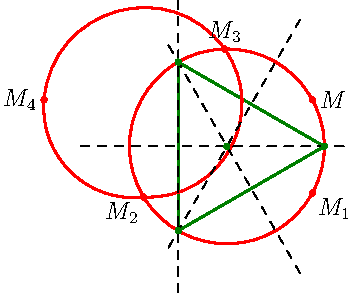
\includegraphics[width=5cm]{Ccomp2_2.pdf}
\caption{$M$ sur le cercle unité} \label{fig:Ccomp2_2}
\end{figure}
\end{enumerate}
